\documentclass[notitlepage,nofootinbib,preprintnumbers,aps,prd]{revtex4-1}
\usepackage{amsmath,amssymb,natbib,bm,color}
\usepackage{graphicx}
\usepackage{placeins}
\graphicspath{ {/Users/alechewitt/Desktop/SULI_paper_images/} }

\newcommand{\comment}[1]{}

\begin{document}

\title{Tracking Stellar Streams Using FAISS}

\author{Alec Hewitt$^1$, Maurice Garcia-Sciveres$^2$, Xiangyang Ju$^2$}
\affiliation{$^1$University of Utah, $^2$Lawrence Berkeley National Laboratory\\
SULI Spring 2021}
%\date{December 2020}

\begin{abstract}
\section*{\underline{Abstract}}
\indent A stellar stream was once a globular cluster or a dwarf galaxy that has been distorted and stretched out due to the tidal forces of a larger galaxy. In particle physics it is useful to know how to trace the trajectories of these interactions. In this project we apply methods of particle physics to locate and track the trajectories of stellar streams. The methods used in this project utilize the machine-learning package “FAISS” (Facebook AI Similarity Search). The algorithm scans the galactic plane for significant clusters, scanning one small dataset at a time. Once these datasets are identified, the algorithm tracks these clusters to determine whether they could be apart of a stellar stream. We found that this can be a promising method for locating and storing information for different stellar streams throughout our galaxy. Information of stellar streams could be helpful for providing evidence on our galaxy’s past as well  as information on our galaxy’s gravitational field.
\end{abstract}
\maketitle


\setlength\parindent{24pt}


\section{\underline{Introduction and Background}}

\indent The Gaia database has data for over 1.8 billion stars. This is only roughly 1-2\% of the stars
contained in the Milky Way but there is still a plethora of data to explore some of the structures
nature can produce. With this amount of data, we cannot rely on traditional programming methods to identify such patterns as this may take an incredibly long time. This is where machine
learning comes in. The main software that will be used is FAISS (Facebook AI Similarity
Search) which is a C++ library but also contains an interface in Python; Python is the language
used in this project. The idea to apply machine learning to astronomical data for this project
came from Maurice Garcia-Sciveres who saw an analogy between particle physics and astro-physics.\\

\indent In particle physics, when particles collide they fly off into particle detectors which detect
the positions of these particles at certain discrete points in space. To know the trajectories they
must “connect the dots” to identify which particles came from where. This is a fairly simple task
to connect the dots for a small number of particles, but once there are thousands of particles,
such tasks become insurmountable. To deal with such a problem, they must figure out a way to
systematically connect the dots. One such method is to take each dot and find the k-nearest
neighbors of that dot, this turns into a combinatorics problem since we are finding every possible
combination of dots and choosing the combinations that correspond to the smallest distances.\\

\indent This can be a computationally intense problem. One way around this is to use a similarity search
that returns the k-nearest neighbors of every particle; such a method requires machine learning.
This project will use a similar technique to analyze data from Gaia eDR3 (2),(3). However, instead of "connecting the dots" of particle trajectories this project provides a tool to connect clusters, where the analogy of a particle in this project is a cluster. Such a tool could be used to locate and map out astronomical objects, such as stellar streams.\\

\indent It is a trivial task to identify whether stars are similar in position, just look at the regions that are clustered.
While these stars may contain similar properties, this project seeks to find clusters of stars in a
similar but more subtle way. Gaia eDR3 has many useful properties that extend beyond just the
position of the star. Only features within the Gaia database identified as “good” measurements
and features that most stars possess are used. Once a dataset has been obtained, the similarity
search can begin. This search involves using the Python package “FAISS” which stands for
“Facebook AI Similarity Search”.\\

\indent A basic example of how this works is as follows: positions of a group of stars are given
within a dataset, the objective is to find the clusters within this data set, i.e., the regions of the
dataset that are the “clumpiest”. FAISS has a function called “Inverted File Index” or “IVF”. This
function takes in the set of vectors, the number of clusters needed, and the number of data points
desired for each cluster and spits out a list of clusters. This project will use a similar method except it will use higher dimensional vectors, however, this particular example can be useful as the
human eye can identify such clusters and this can be used to ensure the methods are returning
intuitively correct results.\\

\indent The research group consists of Maurice Garcia-Sciveres, Xiangyang Ju, and Alec Hewitt.
Maurice is the mentor of this project, Xiangyang is the associate mentor and Alec is the intern.
The purpose of the research group is to have meetings at least once a week to brainstorm. During
these meetings, the intern discusses what progress has been made, possible issues that were encountered, and what can be improved. The mentor and the associate mentor then evaluate the
progress and determine whether the intern is on the right track or whether his methods and direction need to be modified. The results for that week are evaluated and a list of tasks is created to
complete by the next meeting. The intern takes these tasks and attempts to complete them
promptly and regular updates are given throughout the week.\\

\indent Any details that were not covered in the meeting are expanded upon by the intern by using their best judgment. Questions regarding the tasks of the assignment are generally directed
towards the associate mentor while questions regarding the overall direction of the project are
directed towards the mentor.\\


\section{\underline{Methods}}
\indent The goal of this paper is to develop an algorithm to locate a stellar stream and follow it, storing the stars contained within the stream along the way. The first step is to figure out how to locate the stellar stream. Since a stellar stream contains stars traveling in a similar direction, as a first step we can expect that the proper motion of such stars would be clustered in feature space. A more accurate approach would be to locate clusters in proper motion + radial velocity space, but since the measurement of radial velocity is very rare among Gaia data, this feature must be omitted. \\
\section*{Identifying a Stellar Stream}
\indent This algorithm will eventually partition the galaxy into many datasets and search for clusters in each one so this method needs to be a quick way of determining whether there is a possible stream or not. One method would be to cluster the data with N clusters, using the inverted Faiss index and create a plot of number of stars vs. cluster. If there are any pre-clusters that have an unusually high amount of stars within it, this hints that these stars may belong to a cluster, what constitutes an "unusually high amount of stars" is discussed in the results section. \\
	

\section*{Automation }
\indent The next step is to automate this process and a first step is to automate dataset extraction. In order to do this, small datasets are extracted out of the Gaia archive one at a time. To ensure that the same dataset is not analyzed twice an array of points is preselected, each one represents the center of a dataset. This array of points will be referred to as a lattice. The boundaries of the dataset are calculated and they are of the following form
\begin{align*}
	\ell_i - \frac{\Delta \ell}{2} < \ell < \ell_i + \frac{\Delta \ell}{2}\\
	b_j - \frac{\Delta b}{2} < b < b_j + \frac{\Delta b}{2}\\ 
	d_k - \frac{\Delta d_k}{2} < d < d_k + \frac{\Delta d_k}{2},
\end{align*}
where $(\ell_i,b_j,d_k)=(\Delta \ell i, \Delta b j, d_{k-1} + \frac{\Delta d_k}{2} + \frac{\Delta d_{k-1}}{2}) $ represents the center of the $(i,j,k)^{\rm{th}}$ dataset in galactic coordinates and $\Delta d_k = \Delta b (d_{k-1} + \frac{\Delta d_{k-1}}{2})$. Values for $d_0, \Delta d_0, \Delta b$, and $\Delta \ell$ are discussed in the next section. $\ell$ is galactic longitude, $b$ is galactic latitude and $d$ is the distance from the sun to the star. So each lattice point (or center) has a parameter set associated with it.\\
	

\indent The algorithm takes a random point within the lattice as well as its associated parameter set and removes it from the lattice. It uses the parameter set to plug into the Gaia archive to automatically download, retrieve and store the dataset using the python package "selenium" and the software called “chromedriver”. The program then retrieves this from the file and stores it as a dataframe, it then performs the cluster analysis to determine whether the dataset could contain a stream or not. It then takes the information from this analysis and stores it in an array that is in a one to one correspondence with the array of points. This is the process of finding seeds in order to follow the stream. \\

\section*{Following the Stream} 
\indent Once the seeds are found then the algorithm takes all neighboring datasets and analyzes them for stellar streams, if stellar streams are found it keeps searching all boxes around the boxes containing stellar streams until no more stellar streams are found. This has the effect of finding the full cross section of the stream. Then the center of this cross section is determined, a line is fitted to it so that it aims in the direction of the stellar stream and the nearest boxes that it intersects, it analyzes and if it contains a stellar stream, it locates the cross section and keeps repeating this process until the full stellar stream is located.\\

\indent Once the seeds are found the algorithm will then take all neighboring datasets datasets and analyze each of those datasets for clusters, the neighboring datasets of the original seed is referred to as the first layer. If a cluster is found it appends those points to the list of seeds. For each of these seeds, the algorithm will find the neighboring datasets of each of those seeds that have not already been analyzed, this is referred too as the second layer. It will then analyze each of the datasets from the second layer and store the ones that contain clusters. It will then create the neighboring datasets from the 2nd layer, this is called the third layer and so forth. This process continues until there are no more clusters found. This resulting chain of datasets containing clusters may be a part or a whole stellar stream.\\





\section{\underline{Results}}
\indent A cluster is considered to be significant if it contains at least twice the average number of stars and contains more than 120\% of stars than any other cluster in that set. The number of clusters in the data is 50 if the number of stars is less than 10000 and 50 clusters per 10000 stars if the number of stars is greater than 10000 (rounded down). To determine whether the algorithm works, we consider a dataset with a known stellar stream. It is known that there is a stellar stream called GD1 at the location $(x,y,z)=(-1.364, 1.614, 3.204)$ (kpc) \cite{streamfinder}
in galactic coordinates. The positions of stars in this dataset resembles a sector of a sphere and is depicted in Figure \ref{fig:3d_data}.
\FloatBarrier
\begin{figure}[h]
\centering
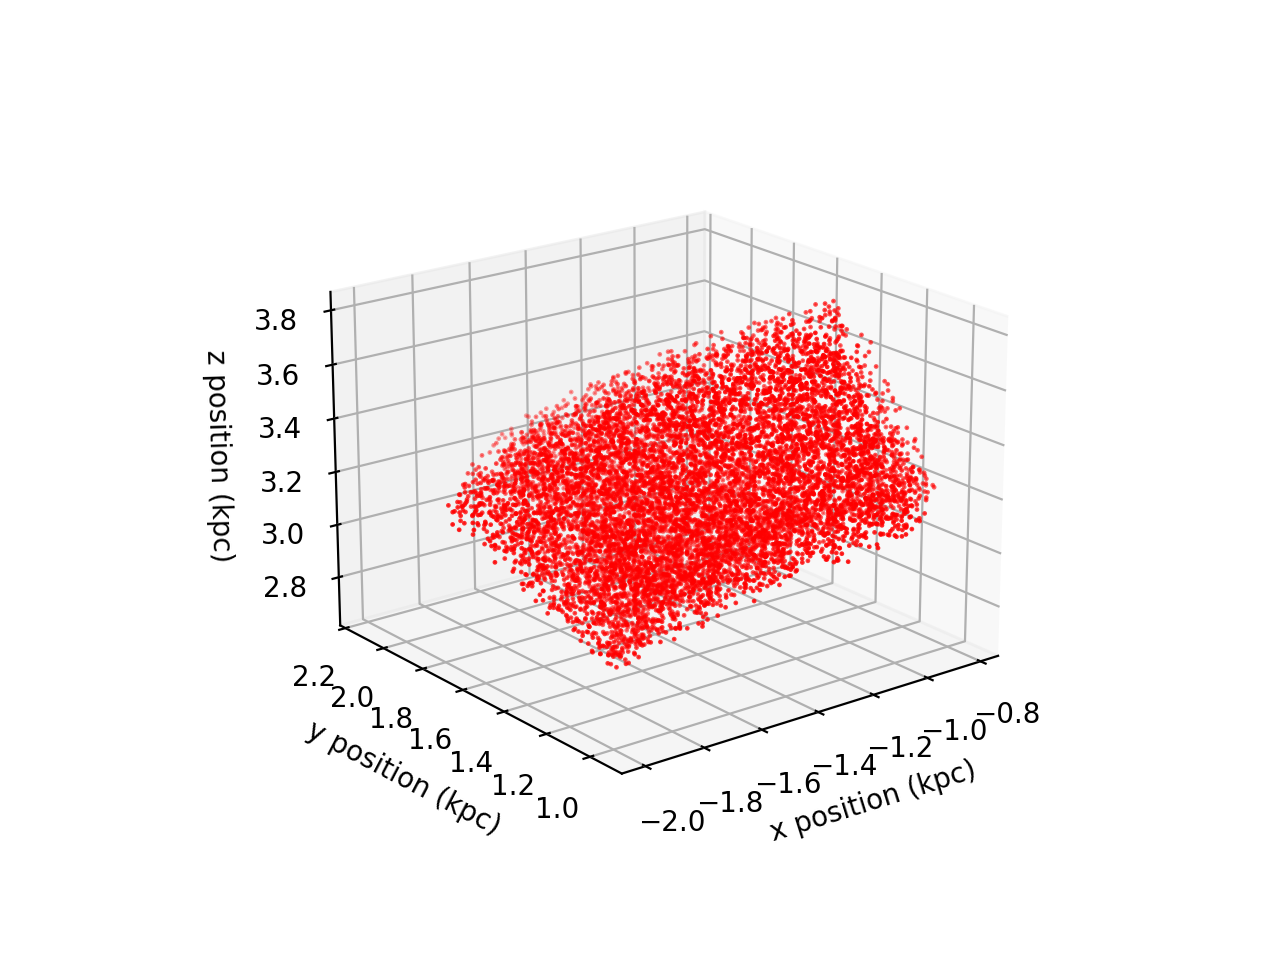
\includegraphics[width=0.5\textwidth]{data_set_2d_new}
\caption{Positions of a 3D dataset; $123.20133060427045<\ell<141.20133060427048$, $50.09349034267207<b<67.09349034267207$, and $3.429787681763778<d<4.17929845130026976$. Center located at $(x,y,z)=(-1.364,1.614,3.204)$ in galactic coordinates}
\label{fig:3d_data}
\end{figure}





If the proper motion of the stars within this region are plotted as in Figure \ref{fig:pmplot}, there is a clear cluster located at roughly $(\mu_{\alpha^*},\mu_{\delta}) \approx (0,0)$ (mas).

\FloatBarrier
\begin{figure}[h]
\centering
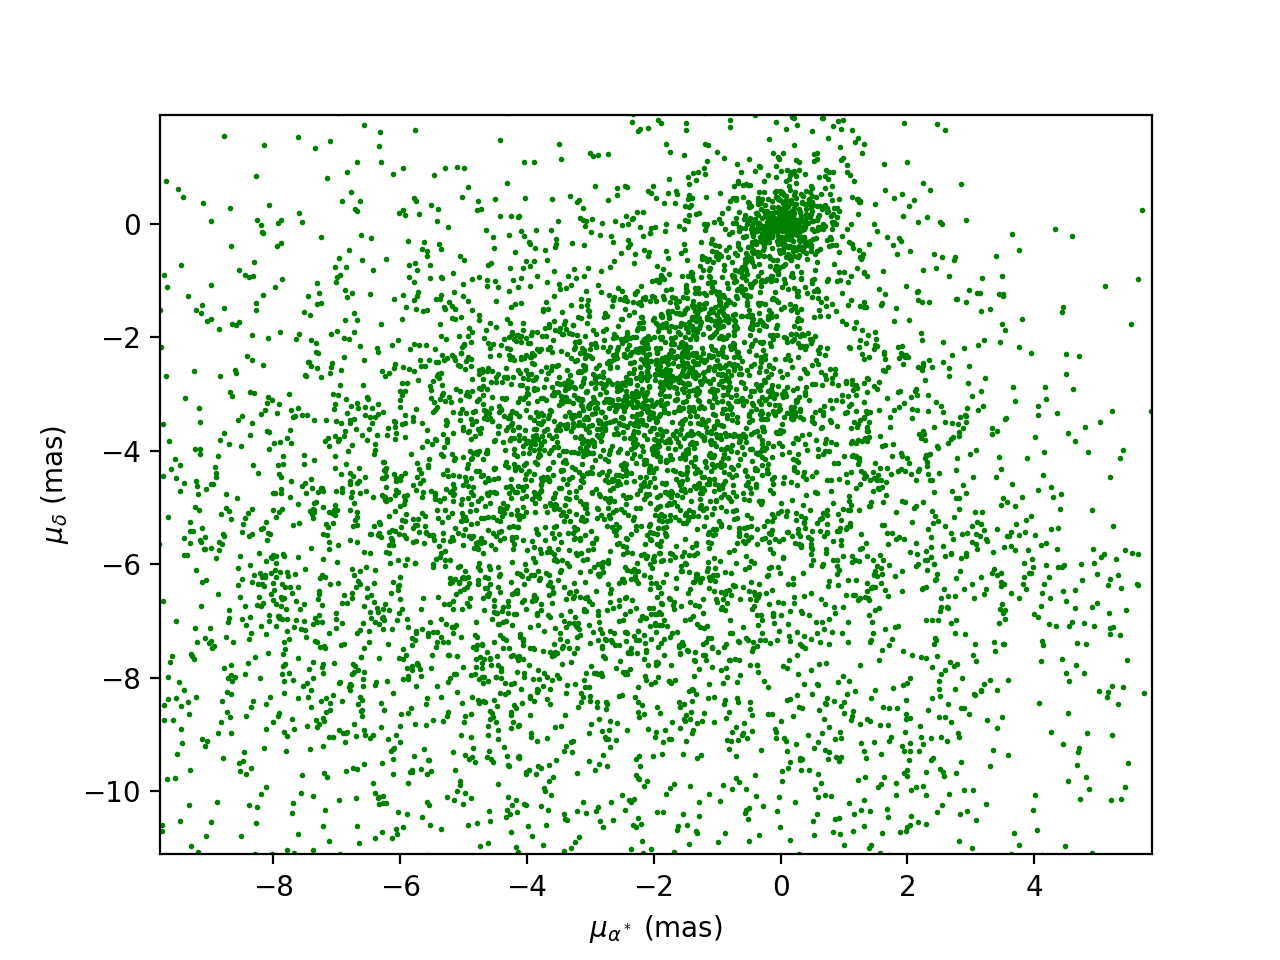
\includegraphics[width=0.5\textwidth]{pm_cluster_new}
\caption{A plot of proper motion showing a cluster at the origin}
\label{fig:pmplot}

\end{figure}





\indent After plotting the number of stars vs. cluster number shown in Figure \ref{fig:numclust}, there is a clear spike in the number of stars, if the cluster corresponding to that spike is extracted and the proper motion is plotted (show plot), it is clear that this is the correct cluster; this is evidence that this method works for identifying streams. This method is a quick way to eliminate datasets that have a low chance of containing a stellar stream and saving a more detailed analysis for the datasets that likely contain a stream. 

\FloatBarrier
\begin{figure}[h]
\centering
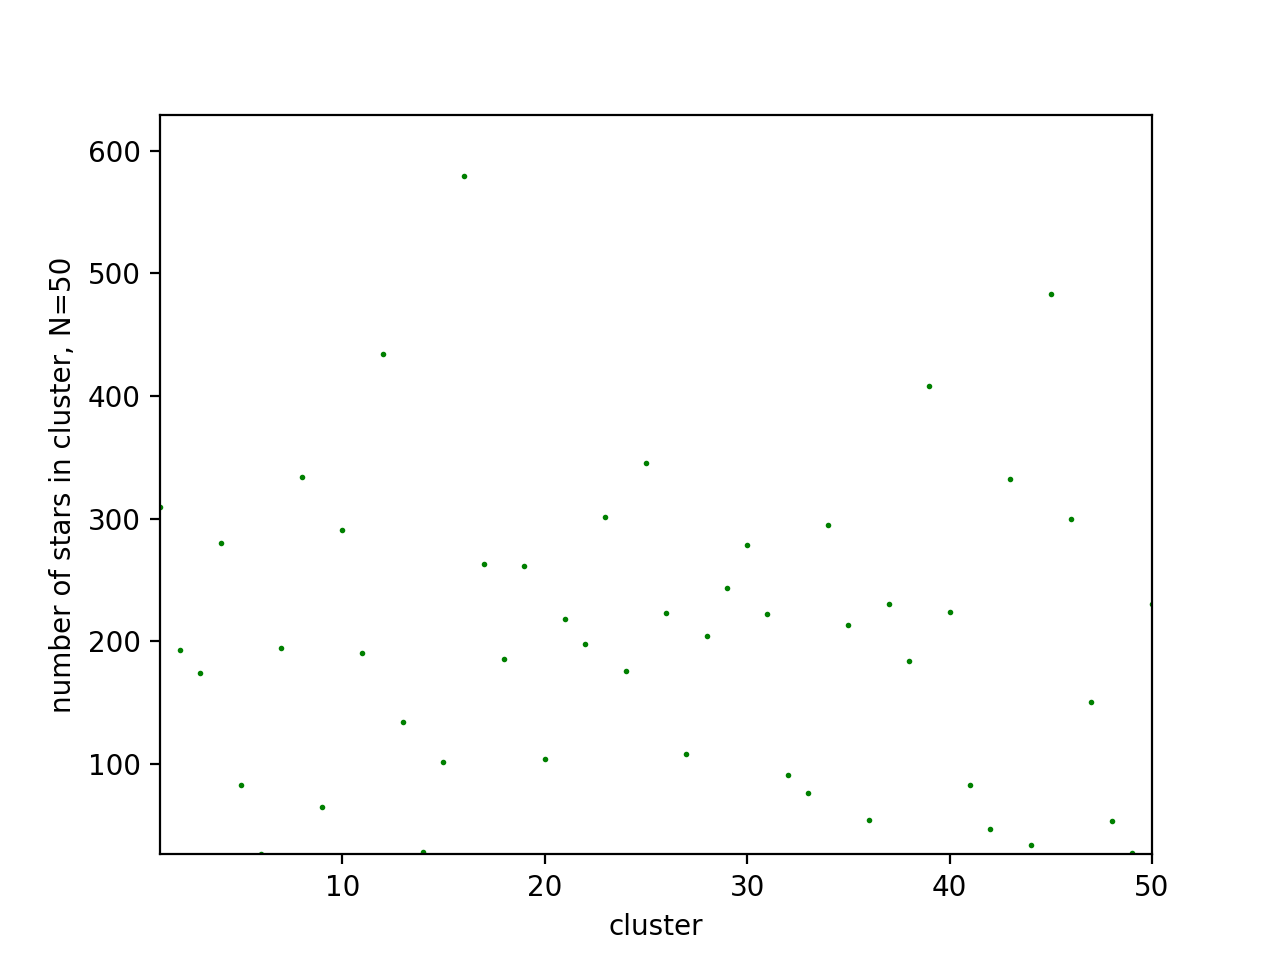
\includegraphics[width=0.5\textwidth]{num_vs_clust_new}
\caption{A plot showing the number of stars in each cluster on the y axis and the corresponding cluster on the x}
\label{fig:numclust}
\end{figure}

\FloatBarrier
\begin{figure}[h]
\centering
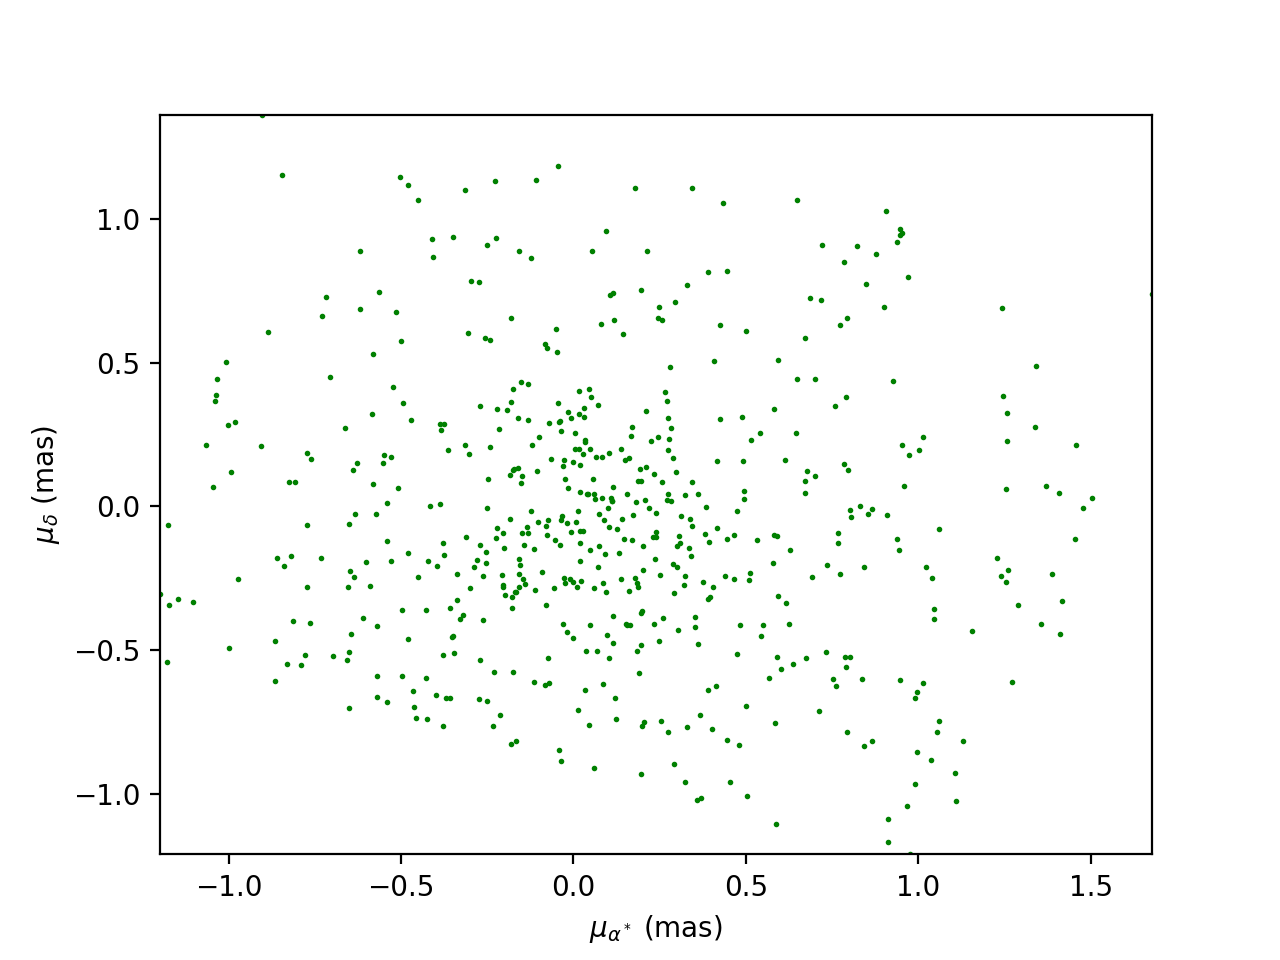
\includegraphics[width=0.5\textwidth]{pm_sig_clust_new}
\caption{A plot of the significant cluster}
\end{figure}

\indent Now that the method is confirmed to work, the results of the overall algorithm is discussed.
As discussed in the methods section, the algorithm preselects points each representing a dataset. We use a disk that is centered at the sun and parallel to the galactic plane. This disk has a radius of roughly 35 kpc is composed of a lattice of each point. We exclude distances that are less than 2 kpc\\
\FloatBarrier
\begin{figure}[h]
\centering
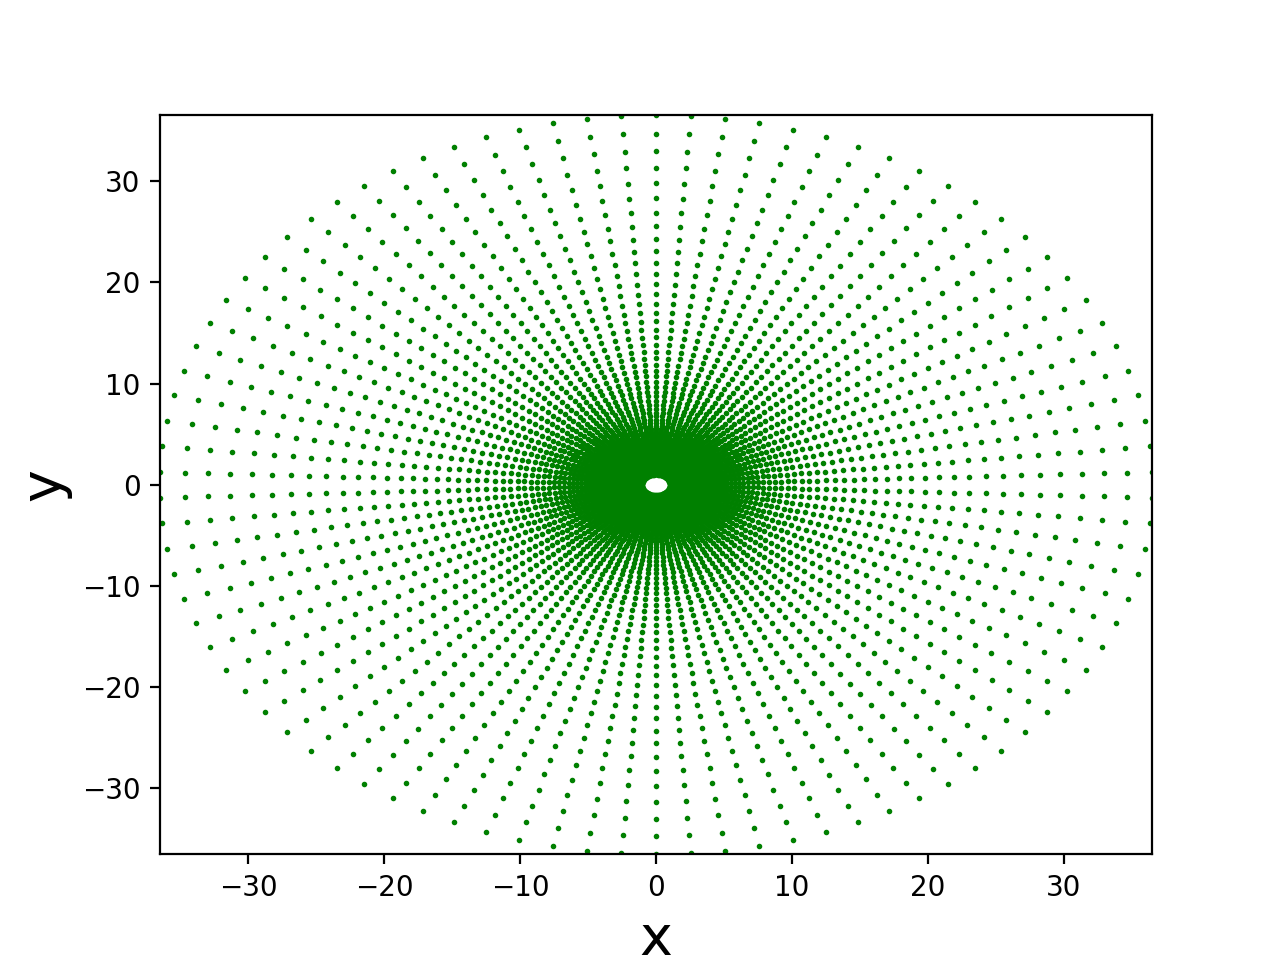
\includegraphics[width=0.5\textwidth]{plane_lattice}
\caption{A lattice of points centered around the sun, each point represents a dataset}
\end{figure}



\indent Here we take $d_0=2 + \frac{\Delta d_0}{2}$, $\Delta d_0=2 \Delta b$, $\Delta b = 3^{\circ}$ and $\Delta l = 4^{\circ}$. The radial thickness has the property that it equals the arc-length of $b$. That is $\Delta d_i = d_{i-1} \Delta b$, where $\Delta b$ is given in radians and $d_i=d_{i-1} + \Delta d_{i-1}$. The width of the block in the radial direction has the property that it equal to the distance created by the arc of b on the initial side.\\
The algorithm scans each of the lattice points one by one for significant clusters. If a significant cluster is found, the algorithm checks all nearest neighbors for stellar streams. To search out of the plane the lattice must be extended into 3-D as a spherical lattice shown in Figure \ref{fig:sphlat}.\\
\FloatBarrier
\begin{figure}[h]
\centering
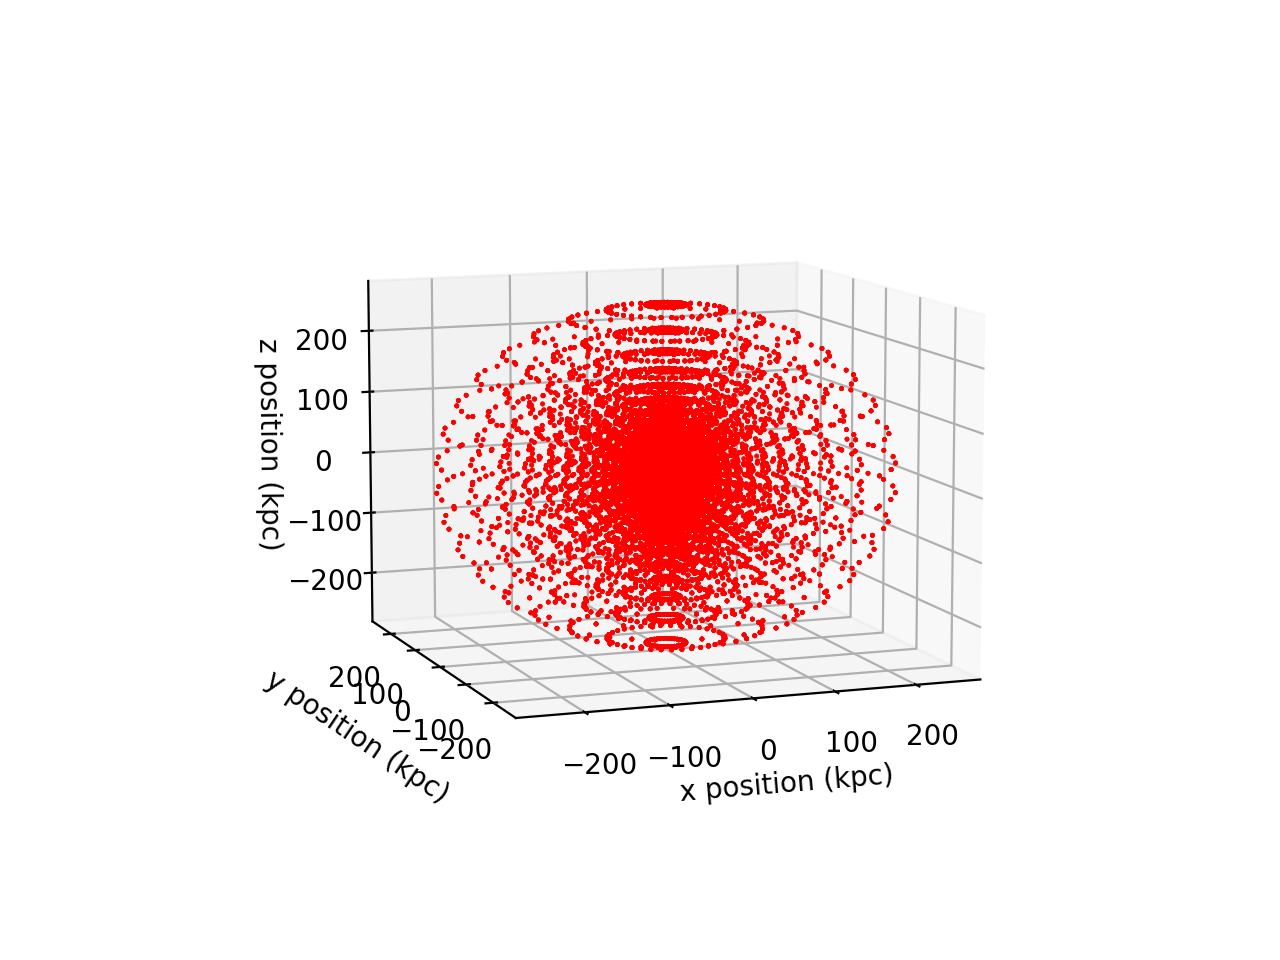
\includegraphics[width=0.5\textwidth]{spherical_lattice}
\caption{A spherical lattice}
\label{fig:sphlat}
\end{figure}

Once a cluster is found, the algorithm searches all nearest neighbors shown in Figure \ref{fig:neigh}.
\FloatBarrier
\begin{figure}[h]
\centering
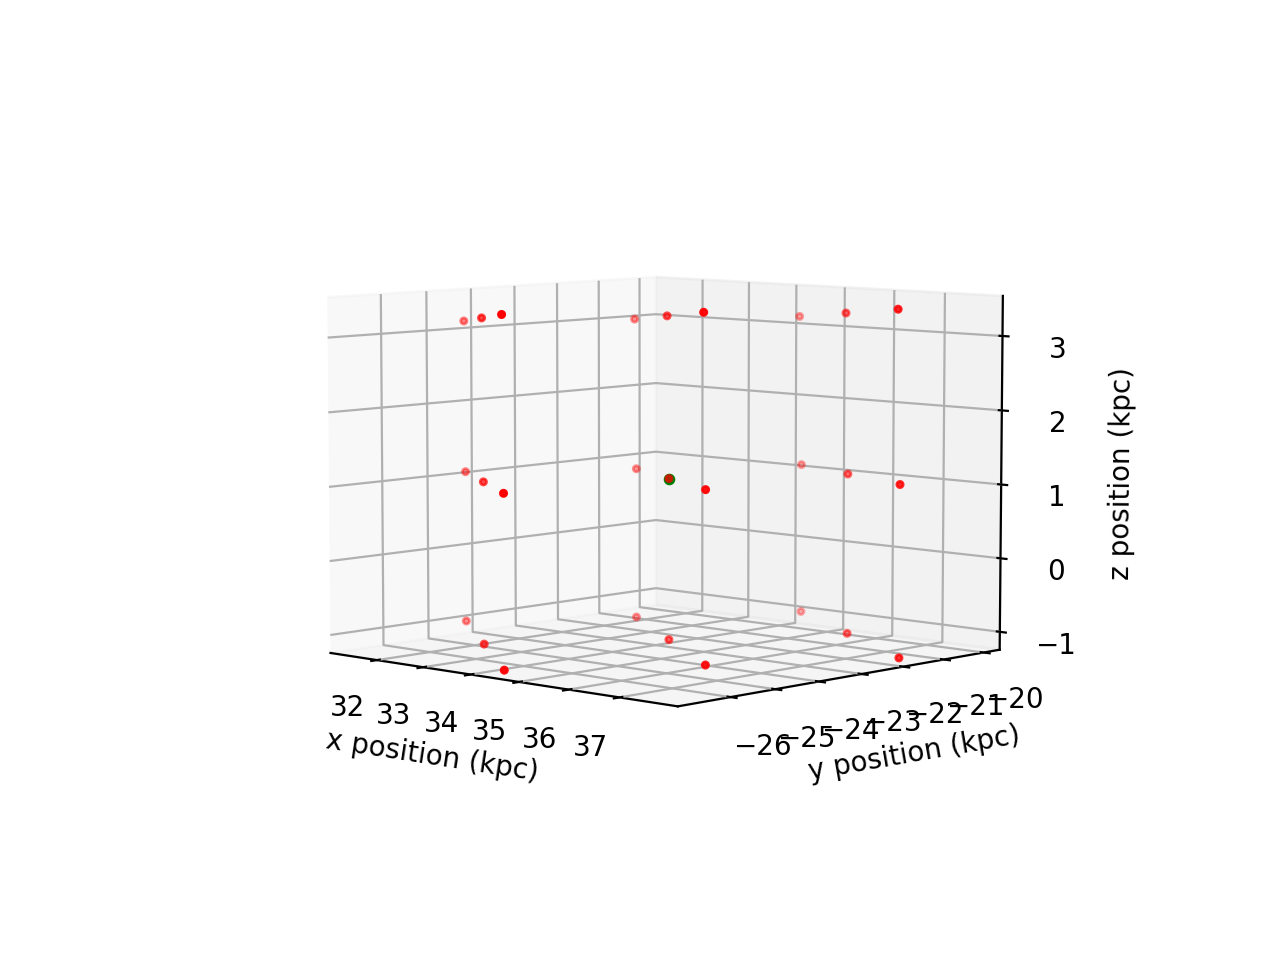
\includegraphics[width=0.5\textwidth]{search_around}
\caption{Neighboring set of a significant dataset, the dark point contains a significant cluster}
\label{fig:neigh}
\end{figure}

If a neighbor contains a significant cluster, this process is repeated as discussed previously.


\section{\underline{Discussion}}
\indent The methods discussed provide a promising tool to locate and track clusters. When a cluster is present the plots of “number of stars vs. clusters” illustrate a clear peak, this peak corresponds to a cluster. When there is no cluster present there is no longer a peak that sticks out clearly and the algorithm will indicate this. \\

\indent The algorithm designed to scan the galactic plane must scan thousands of datasets, each dataset can take several minutes. Furthermore, when a seed for the cluster is found, tracking the cluster involves scanning 26 datasets around the dataset containing the cluster and for each of those it scans all neighboring datasets that have not been previously analyzed. This process can be very time consuming as well. An obvious improvement to this algorithm would be to incorporate multiprocessing. This would allow the algorithm that scans the galactic plane to become increasingly fast, depending on how many cores the machine possesses. The algorithm that tracks can be made much faster as well  since instead of scanning all neighboring datasets one by one, each neighboring dataset can be given to a separate core and scan of each layer could equal the same amount of time as just scanning a single dataset.\\

\indent This program works for larger radii, currently it works best for distances exceeding 2 kpc from the sun. This was an unexpected difficulty. Datasets that are close to the sun all possess clusters. These clusters are centered at (0,0) which suggests they are traveling in the same direction as the sun. A possible reason for this tight cluster is due to the distance from the sun. For small distances it can be common for the angular velocity to exceed 100 mas/yr whereas for larger distances large angular velocities become exceedingly rare. A solution would be to exclude clusters whose centers are close to (0,0).

\section{Conclusion}
\indent The purpose of this project was to determine whether an algorithm could be constructed that could successfully identify and track stellar streams. The methods presented show promising results that this is possible with some caveats. The methods work for radii larger than 2 kpc and can scan the galactic plane for significant clusters, choosing one dataset at a time. The algorithm has a separate function that can take in potential candidates and track these clusters. This could be improved by including radii less than 2 kpc as a special case. Currently the algorithm needs more testing in order to improve the constraints for determining a significant cluster. The algorithm is designed for a single core, however, a few simple modifications could allow for multiprocessing.\\
\section{Acknowledgements}
This work was supported in part by the U.S. Department of Energy, Office of Science, Office of Workforce Development for Teachers and Scientists (WDTS) under the Science Undergraduate Laboratory Internship (SULI) program. 
This work has made use of data from the European Space Agency (ESA) mission
{\it Gaia} (\url{https://www.cosmos.esa.int/gaia}), processed by the {\it Gaia}
Data Processing and Analysis Consortium (DPAC,
\url{https://www.cosmos.esa.int/web/gaia/dpac/consortium}). Funding for the DPAC
has been provided by national institutions, in particular the institutions
participating in the {\it Gaia} Multilateral Agreement.
	




\section{References}
\begin{thebibliography}{99}

\bibitem{gaia_examples}
\textit{ https://gea.esac.esa.int/archive-help/adql/examples/index.html}
\bibitem{gaia_mission}
\textit{Gaia Collaboration et al. (2016b): The Gaia mission (provides a description of the Gaia mission including spacecraft, instruments, survey and measurement principles, and operations)}
\bibitem{gaia_summary}
\textit{Gaia Collaboration et al. (2020b): Gaia EDR3: Summary of the contents and survey properties.}
\bibitem{sklearn}
\textit{F. Pedregosa, G. Varoquaux, A. Gramfort, V. Michel, B. Thirion, O. Grisel, M. Blondel, P. Prettenhofer, R. Weiss, V. Dubourg, J. Vander- plas, A. Passos, D. Cournapeau, M. Brucher, M. Perrot, and E. Duch- esnay. Scikit-learn: Machine learning in Python. Journal of Machine Learning Research, 12:2825–2830, 2011.}
\bibitem{streamfinder}
\textit{Rodrigo A. Ibata, Khyati Malhan, and Nicolas F. Martin. The streams of the gaping abyss: A population of entangled stellar streams surrounding the inner galaxy. The Astrophysical Journal, 872(2):152, 2019.}

\end{thebibliography}




\end{document}
